\section{调用Xilinx库Block Memory Generator方法}\label{section:section_2}
\subsection{新建工程}
新建一个工程 data\_ram, 参考文档“A04\_Vivado使用说明” :
\begin{figure}[htbp]
    \centering
    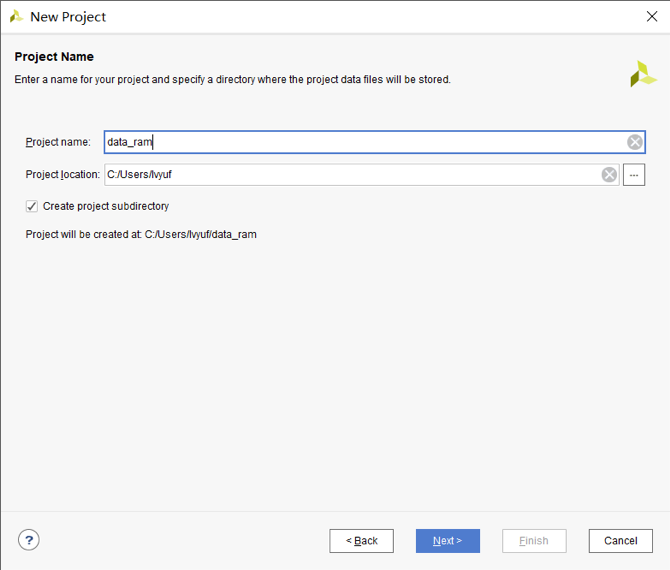
\includegraphics[width = 0.65\textwidth]{image/2_section/section_2_0.png}
    \caption{新建工程}
    \label{fig:section_2_0}
\end{figure}
\subsection{新建IP}
IP核查找路径:Flow Navigator->IP Catalog->Vivado Repository ->Basic Elements->Memory Elements->Block Memory Generator
\begin{figure}[htbp]
    \centering
    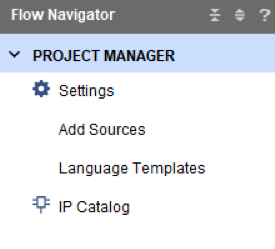
\includegraphics[width = 0.3\textwidth]{image/2_section/section_2_1.png}
    \caption{查找IP}
    \label{fig:section_2_1}
\end{figure}

或者Flow Navigator->IP Catalog,在搜索栏直接搜索Block Memory Generator

\begin{figure}[htbp]
    \centering
    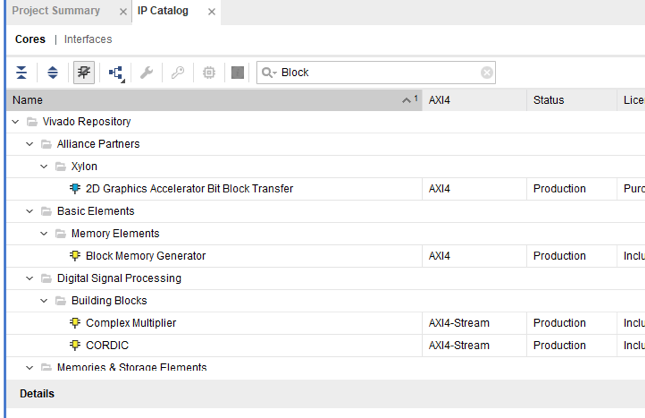
\includegraphics[width = 0.65\textwidth]{image/2_section/section_2_2.png}
    \caption{搜索Block Memory Generator}
    \label{fig:section_2_2}
\end{figure}

\subsection{设置RAM参数}
Block Memory Generator共有四类设置,分别为Basic、端口设置、其他设置、Summary:
\begin{figure}[htbp]
    \centering
    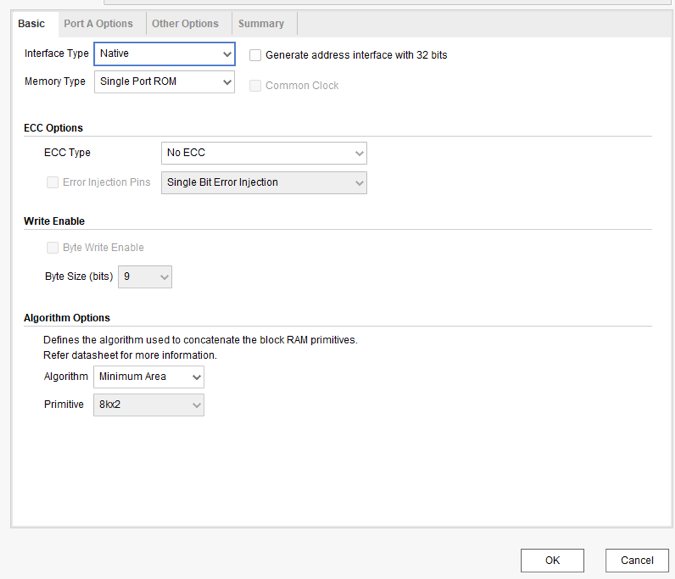
\includegraphics[width = 0.65\textwidth]{image/2_section/section_2_3.png}
    \caption{Basic}
    \label{fig:section_2_3}
\end{figure}

其中Basic需要设置存储器类型,Interface Type需选择Native,选中Generate address interface with 32bits,将地址长度设置为32位,Memory Type根据实验要求选择,其他选项无需设置。

\begin{figure}[htbp]
    \centering
    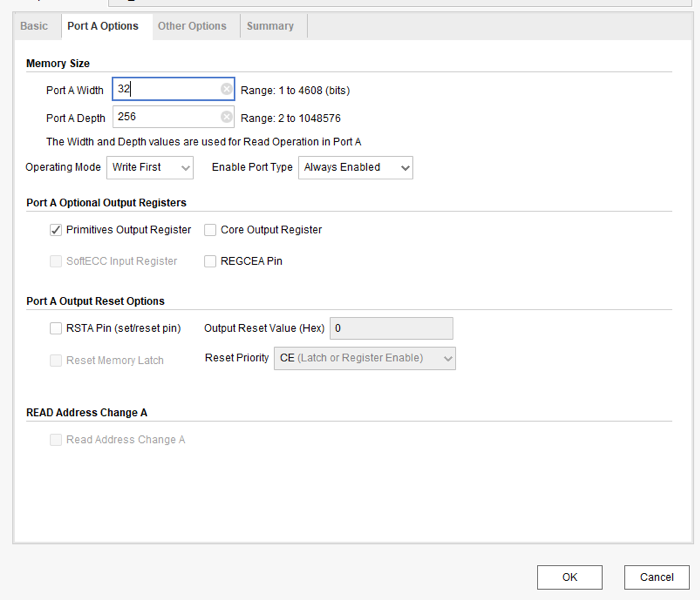
\includegraphics[width = 0.65\textwidth]{image/2_section/section_2_4.png}
    \caption{端口设置}
    \label{fig:section_2_4}
\end{figure}

端口设置需要设置数据字宽度及阵列深度,根据实验要求,字宽均为32位,阵列深度需根据需求自定义,但不可超过155520字。

写数据端口默认开启写使能,读数据端口默认不开启,可根据自己需求选择Enable Port Type。

\subsection{设置初始化数据}
\begin{figure}[htbp]
    \centering
    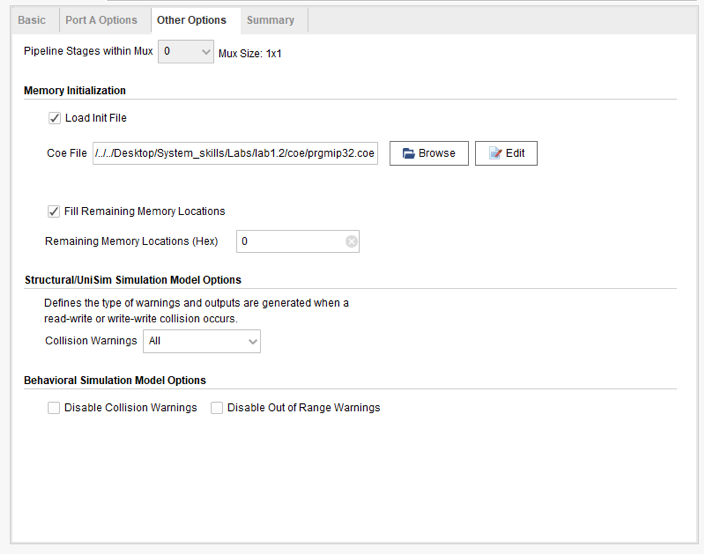
\includegraphics[width = 0.65\textwidth]{image/2_section/section_2_5.png}
    \caption{设置初始化数据}
    \label{fig:section_2_5}
\end{figure}

其他设置主要用于加载coe文件,在图~\ref{fig:section_2_5}中,需要勾选“Load Init File”,并选中需要装载的初始化文件(.coe 文件)。 .coe 文件为 Vivado 中存储器初始化文件,其格式如下:
\begin{lstlisting}[numbers=left,xleftmargin=5em,xrightmargin=5em, aboveskip=2em]
memory_initialization_radix = 16;
memory_initialization_vector =
24010001
00011100
……
\end{lstlisting}

第一行指定了初始化数据格式,此处为 16 进制,也可以设置为 2 进制。第二行说明从第三行开始为初始化的数据向量,由于宽度为 32 位,故一个初始化向量为 32 位数据。初始化向量之间必须用空格或换行符隔开,此处使用换行符,故一行为一个初始化向量。初始化数据会从 RAM 中的 0 地址处开始依次填充。当初始化数据格式设置为 2 进制时,后续的初始化向量需要用二进制编写。

这里只需要注意一个问题,Fill Remaining Memory Locations需要选中,以防读数据操作时,地址超过coe文件已有数据范围,导致异常。